\documentclass[12pt]{article}

\usepackage[a4paper,margin=1in]{geometry}
\usepackage{amsmath,amssymb}
\usepackage{newtxtext,newtxmath} % Times-style font
\usepackage{fancyhdr}
\usepackage{listings}
\usepackage{graphicx}
\usepackage{float}
\usepackage{algorithm}
\usepackage{algpseudocode}
\usepackage{xcolor}
\usepackage{booktabs}
\usepackage{array}

\setlength{\textfloatsep}{10pt}
\setlength{\floatsep}{10pt}

\setlength{\parindent}{0pt}
\setlength{\parskip}{5pt}

% Keep entire document at 12 pt
\AtBeginDocument{
    \fontsize{12pt}{14pt}\selectfont
}

\lstdefinestyle{code}{
    language=Python,
    basicstyle=\ttfamily\fontsize{9.5pt}{11.5pt}\selectfont,
    breaklines=true,
    breakatwhitespace=false,
    frame=single,
    numbers=left,
    numberstyle=\tiny\color{gray},
    keywordstyle=\color{blue},
    commentstyle=\color{gray},
    stringstyle=\color{green!50!black},
    columns=fullflexible,
    keepspaces=true,
    showstringspaces=false
}

\lstdefinestyle{output}{
    basicstyle=\ttfamily\fontsize{9.5pt}{11.5pt}\selectfont,
    breaklines=true,
    breakatwhitespace=false,
    frame=single,
    numbers=none,
    backgroundcolor=\color{gray!6},
    columns=fullflexible,
    keepspaces=true,
    showstringspaces=false
}

% ------------------------------------------------
% Header
% ------------------------------------------------

\pagestyle{fancy}
\fancyhf{}

\fancyhead[L]{Name: Kishan Sahu{\hspace{6cm}}}
\fancyhead[R]{Enrollment No.: P26DS017}

\renewcommand{\headrulewidth}{0.4pt}
\setlength{\headheight}{15pt}

\begin{document}

% ------------------------------------------------
% TITLE
% ------------------------------------------------

\begin{center}
\textbf{Computer Science and Engineering Department, SVNIT, Surat}\\
\textbf{M.Tech. I -- Semester I}\\
\textbf{Computer Vision and Image Processing (CSCS111/CSDS119)}\\
\textbf{Lab Assignment 8}\\
\textbf{Motion Analysis}
\end{center}
\vspace{-4pt}
\hrule
\vspace{6pt}

\section{Introduction and Problem Statement}
Motion analysis is a fundamental task in computer vision, widely used in video surveillance, traffic monitoring, and automated activity recognition. In this assignment, we analyze a corridor surveillance recording (\texttt{motion\_corridor.avi}) featuring two individuals walking through a corridor. 

\textbf{Core Objectives:}
\begin{enumerate}
    \item Load the video, retrieve and display video metadata (frame count, dimensions, frame rate), extract sample frames, convert them to grayscale, and observe inter-frame intensity changes.
    \item Implement \textbf{Frame Differencing} and \textbf{MOG2 Background Subtraction} (\texttt{cv2.createBackgroundSubtractorMOG2()}), and evaluate the impact of various threshold settings on motion detection masks.
    \item Compare both motion detection techniques on video segments where a person halts or illumination changes abruptly.
    \item Address the \textbf{Challenge Question}: Can motion detectors distinguish a stationary person from the background? Provide evidence from the video and propose concrete algorithmic improvements.
\end{enumerate}

\section{Methodology and Theoretical Background}

\subsection{Frame Differencing}
Given consecutive grayscale video frames $I_t(x, y)$ and $I_{t-1}(x, y)$, the inter-frame difference $D_t(x, y)$ is calculated as the absolute intensity discrepancy:
\begin{equation}
    D_t(x, y) = |I_t(x, y) - I_{t-1}(x, y)|
\end{equation}
A binary motion mask $M_{\text{FD}}(x, y)$ is obtained by thresholding with value $T$:
\begin{equation}
    M_{\text{FD}}(x, y) = 
    \begin{cases} 
        255, & \text{if } D_t(x, y) \ge T \\
        0, & \text{otherwise}
    \end{cases}
\end{equation}
\textbf{Properties:} Highly computationally efficient ($O(1)$ temporal memory), but only detects motion occurring \emph{between the immediate two frames}. If an object becomes stationary, $D_t(x, y) \to 0$, causing the object to disappear from the detection mask.

\subsection{Gaussian Mixture-based Background Subtraction (MOG2)}
The MOG2 algorithm models the background history of each individual pixel as a mixture of $K$ adaptive Gaussians:
\begin{equation}
    P(X_t) = \sum_{i=1}^K \omega_{i, t} \cdot \eta(X_t, \mu_{i, t}, \Sigma_{i, t})
\end{equation}
where $\omega_{i, t}$ is the mixture weight, and $\eta(X_t, \mu_{i, t}, \Sigma_{i, t})$ is the multivariate normal probability density. The parameter $K$ dynamically adapts per pixel depending on scene complexity. Pixels deviating by more than a threshold variance ($c_t = 2.5\sigma$) from the background distributions are flagged as foreground.

\subsection{Motion Vector Estimation and Optical Flow Constraint}
Optical flow computes the apparent motion field between consecutive video frames under the Brightness Constancy assumption:
\begin{equation}
    I(x + u, y + v, t + 1) \approx I(x, y, t)
\end{equation}
Linearizing via first-order Taylor expansion yields the Optical Flow Constraint Equation:
\begin{equation}
    I_x u + I_y v + I_t = 0 \quad \iff \quad \nabla I \cdot \vec{V} + I_t = 0
\end{equation}
where $\nabla I = [I_x, I_y]^T$ represents spatial intensity gradients, $I_t \approx I_{t+1}(x,y) - I_t(x,y)$ is the temporal derivative, and $\vec{V} = [u, v]^T$ is the motion vector. The normal velocity measurable along the local gradient is:
\begin{equation}
    \vec{V}_n = -\frac{I_t}{\|\nabla I\|}\frac{\nabla I}{\|\nabla I\|} \implies \|\vec{V}_n\| = \frac{|I_t|}{\|\nabla I\|}
\end{equation}
Due to the Aperture Problem, movement parallel to intensity edges ($\nabla I \perp \vec{V}$) cannot be resolved from local gradients alone. Dense polynomial expansion (Farneback's algorithm) solves this by approximating neighborhoods with quadratic polynomials. Each 2D displacement vector $(u, v)$ is converted to polar coordinates:
\begin{align}
    \text{Magnitude (Speed): } & r = \sqrt{u^2 + v^2} \\
    \text{Direction (Orientation): } & \theta = \arctan2(v, u) \in [0^\circ, 360^\circ)
\end{align}
Direction is visualized continuously via dense HSV color encoding ($\text{Hue} \propto \theta$, $\text{Value} \propto r$) and sparse vector quiver plots.

\section{Implementation and Experimental Results}

\subsection{Task 1: Video Loading, Metadata, and Frame Observation}
The video \texttt{motion\_corridor.avi} is loaded using \texttt{cv2.VideoCapture}. Frames are read and converted to grayscale, and consecutive frame changes are visualized.

\begin{lstlisting}[style=code, caption={Loading video and inspecting metadata}]
import cv2
import numpy as np
import matplotlib.pyplot as plt

# 1. Load video and retrieve metadata
video_path = 'motion_corridor.avi'
cap = cv2.VideoCapture(video_path)

if not cap.isOpened():
    raise IOError(f"Cannot open video file: {video_path}")

total_frames = int(cap.get(cv2.CAP_PROP_FRAME_COUNT))
fps = cap.get(cv2.CAP_PROP_FPS)
width = int(cap.get(cv2.CAP_PROP_FRAME_WIDTH))
height = int(cap.get(cv2.CAP_PROP_FRAME_HEIGHT))

print("Video Metadata:")
print(f" - Total Frames : {total_frames}")
print(f" - FPS          : {fps}")
print(f" - Resolution   : {width} x {height}")

frames = []
while True:
    ret, frame = cap.read()
    if not ret:
        break
    frames.append(frame)
cap.release()

gray_frames = [cv2.cvtColor(f, cv2.COLOR_BGR2GRAY) for f in frames]
\end{lstlisting}

\begin{lstlisting}[style=output, caption={Console Output: Video Metadata}]
Video Metadata:
 - Total Frames : 96
 - FPS          : 12.0
 - Resolution   : 640 x 360
\end{lstlisting}

\begin{figure}[H]
    \centering
    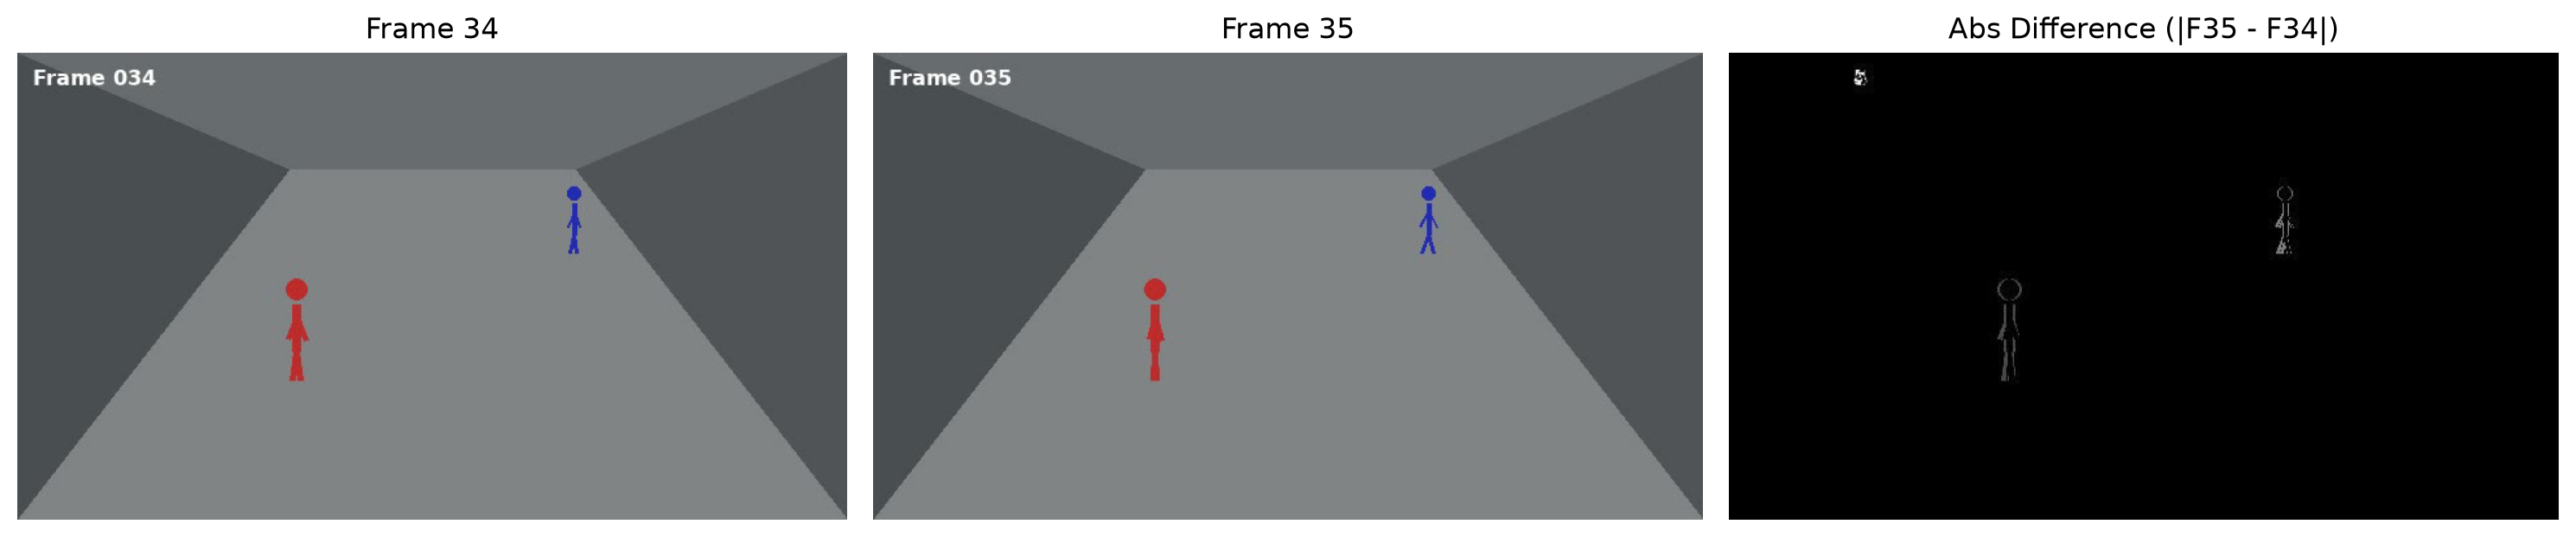
\includegraphics[width=0.95\textwidth]{images/consecutive_diff.png}
    \caption{Consecutive frames (Frame 34 and Frame 35) and their absolute grayscale difference mask $|F_{35} - F_{34}|$.}
    \label{fig:consecutive_diff}
\end{figure}

\subsection{Task 2: Frame Differencing vs. MOG2 and Threshold Sensitivity}
We evaluate the sensitivity of the binary threshold $T \in \{15, 30, 60\}$ in inter-frame differencing, and compare the result against the foreground mask generated by MOG2.

\begin{lstlisting}[style=code, caption={Frame differencing with varying thresholds and MOG2}]
def frame_difference_mask(prev_gray, curr_gray, threshold_val=30):
    diff = cv2.absdiff(curr_gray, prev_gray)
    _, mask = cv2.threshold(diff, threshold_val, 255, cv2.THRESH_BINARY)
    return diff, mask

# Threshold sensitivity evaluation on Frame 35
thresholds = [15, 30, 60]
for idx, t in enumerate(thresholds):
    _, mask = frame_difference_mask(gray_frames[34], gray_frames[35], threshold_val=t)

# MOG2 Background Subtraction
fgbg = cv2.createBackgroundSubtractorMOG2(history=50, varThreshold=25, detectShadows=True)
mog2_masks = [fgbg.apply(frame) for frame in frames]
\end{lstlisting}

\begin{figure}[H]
    \centering
    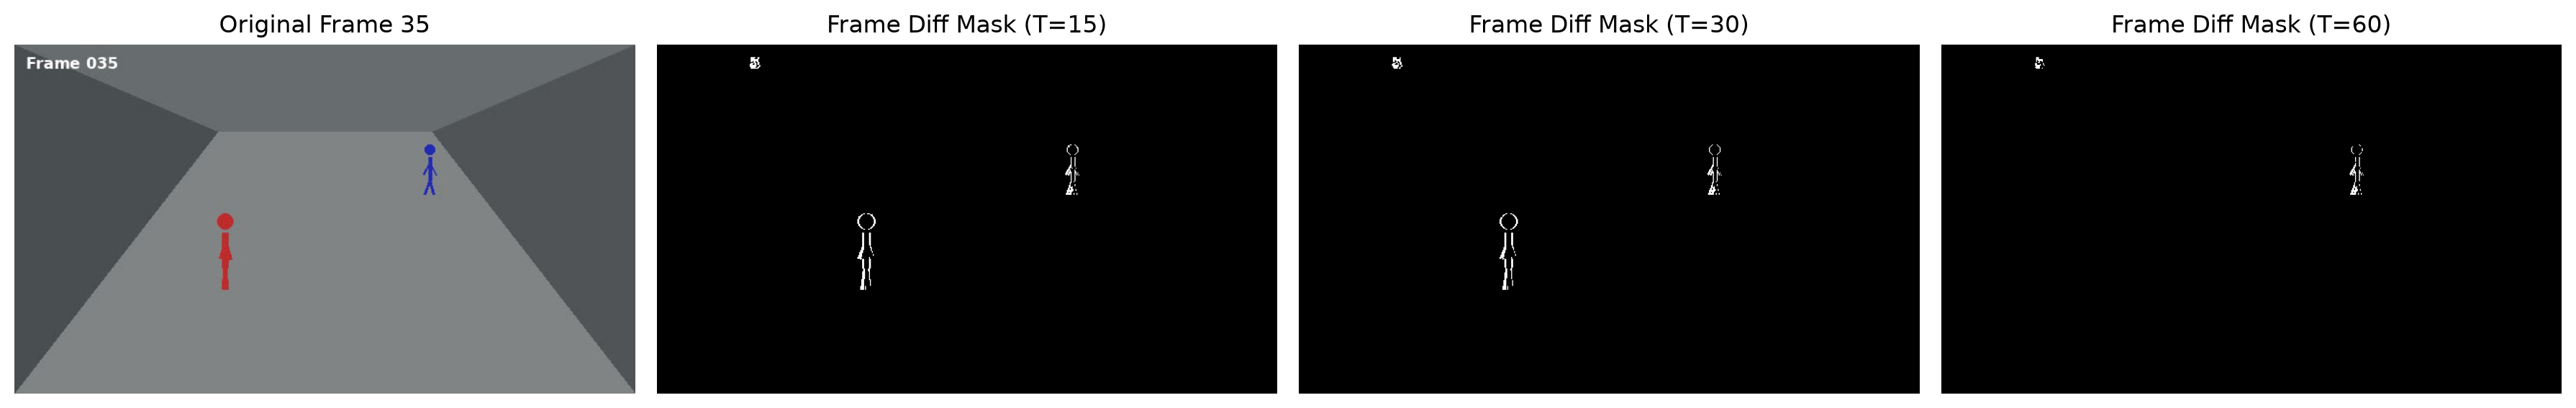
\includegraphics[width=0.98\textwidth]{images/threshold_comparison.png}
    \caption{Comparison of frame differencing masks across thresholds $T = 15, 30, 60$ on Frame 35.}
    \label{fig:threshold_comparison}
\end{figure}

\begin{figure}[H]
    \centering
    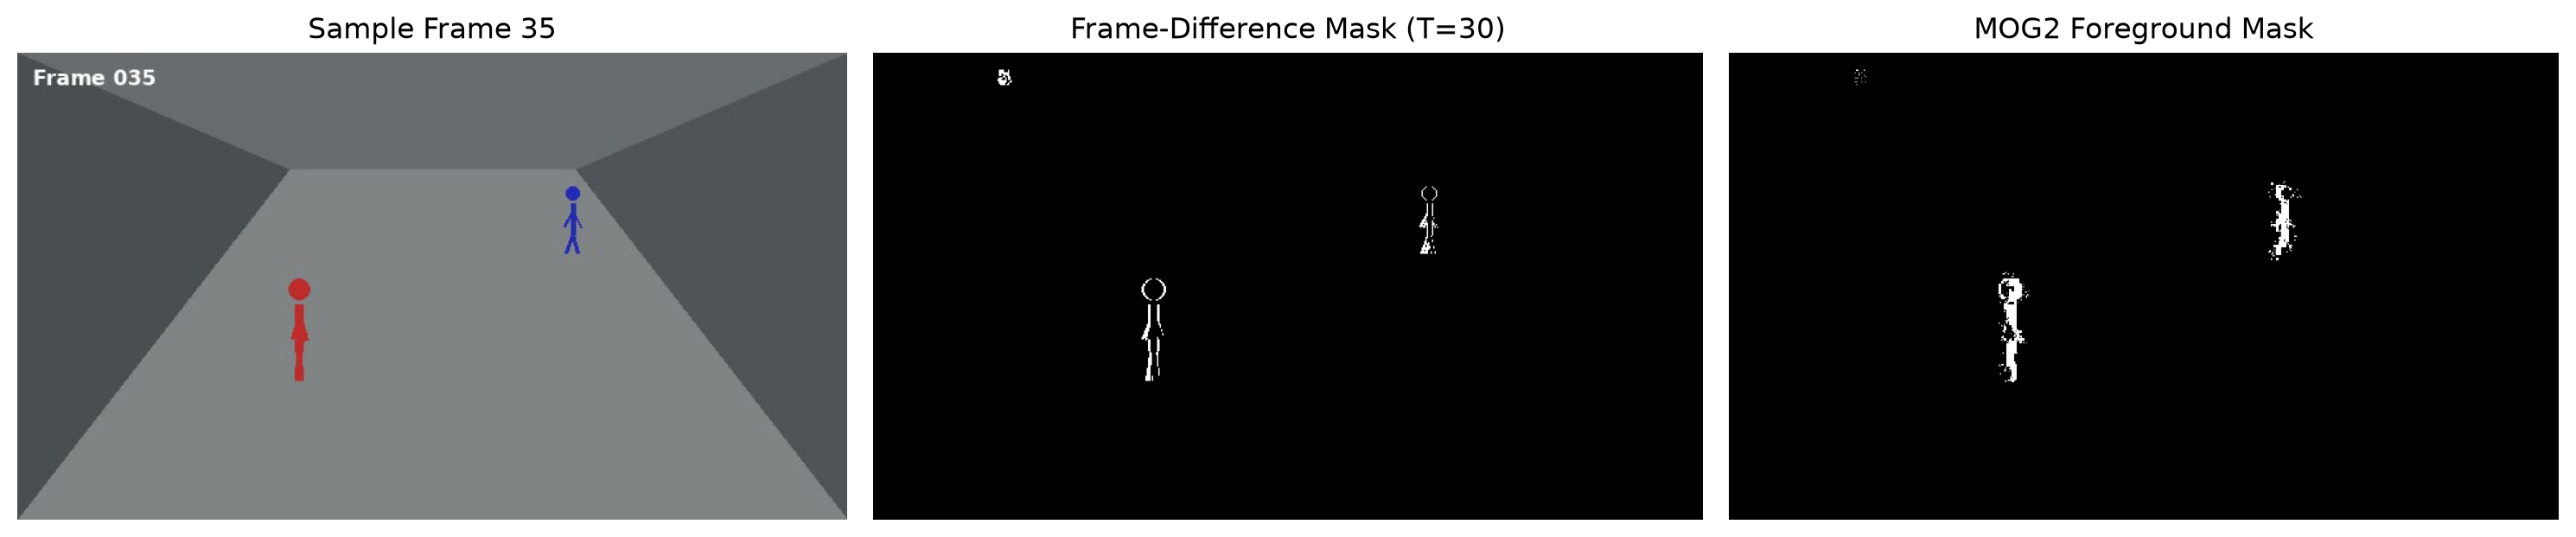
\includegraphics[width=0.95\textwidth]{images/mog2_vs_framediff.png}
    \caption{Sample Frame 35: Comparison between Frame Differencing ($T=30$) and MOG2 Background Subtraction.}
    \label{fig:mog2_vs_framediff}
\end{figure}

\textbf{Observations on Threshold Settings:}
\begin{itemize}
    \item \textbf{Low Threshold ($T=15$):} Captures extensive foreground contours but introduces sensor and compression noise along the floor and wall shadows.
    \item \textbf{Medium Threshold ($T=30$):} Balances noise suppression with reliable boundary detection for moving subjects.
    \item \textbf{High Threshold ($T=60$):} Completely suppresses noise, but the detected silhouettes become broken, fragmented, and lose lower-contrast body regions.
\end{itemize}

\subsection{Task 3: Comparative Evaluation on Paused Motion and Illumination Shift}
In the corridor footage:
\begin{itemize}
    \item \textbf{Around Frame 62:} The red subject on the left comes to a complete halt while the blue subject continues moving.
    \item \textbf{At Frame 70:} An abrupt illumination surge occurs across the corridor.
\end{itemize}

\begin{figure}[H]
    \centering
    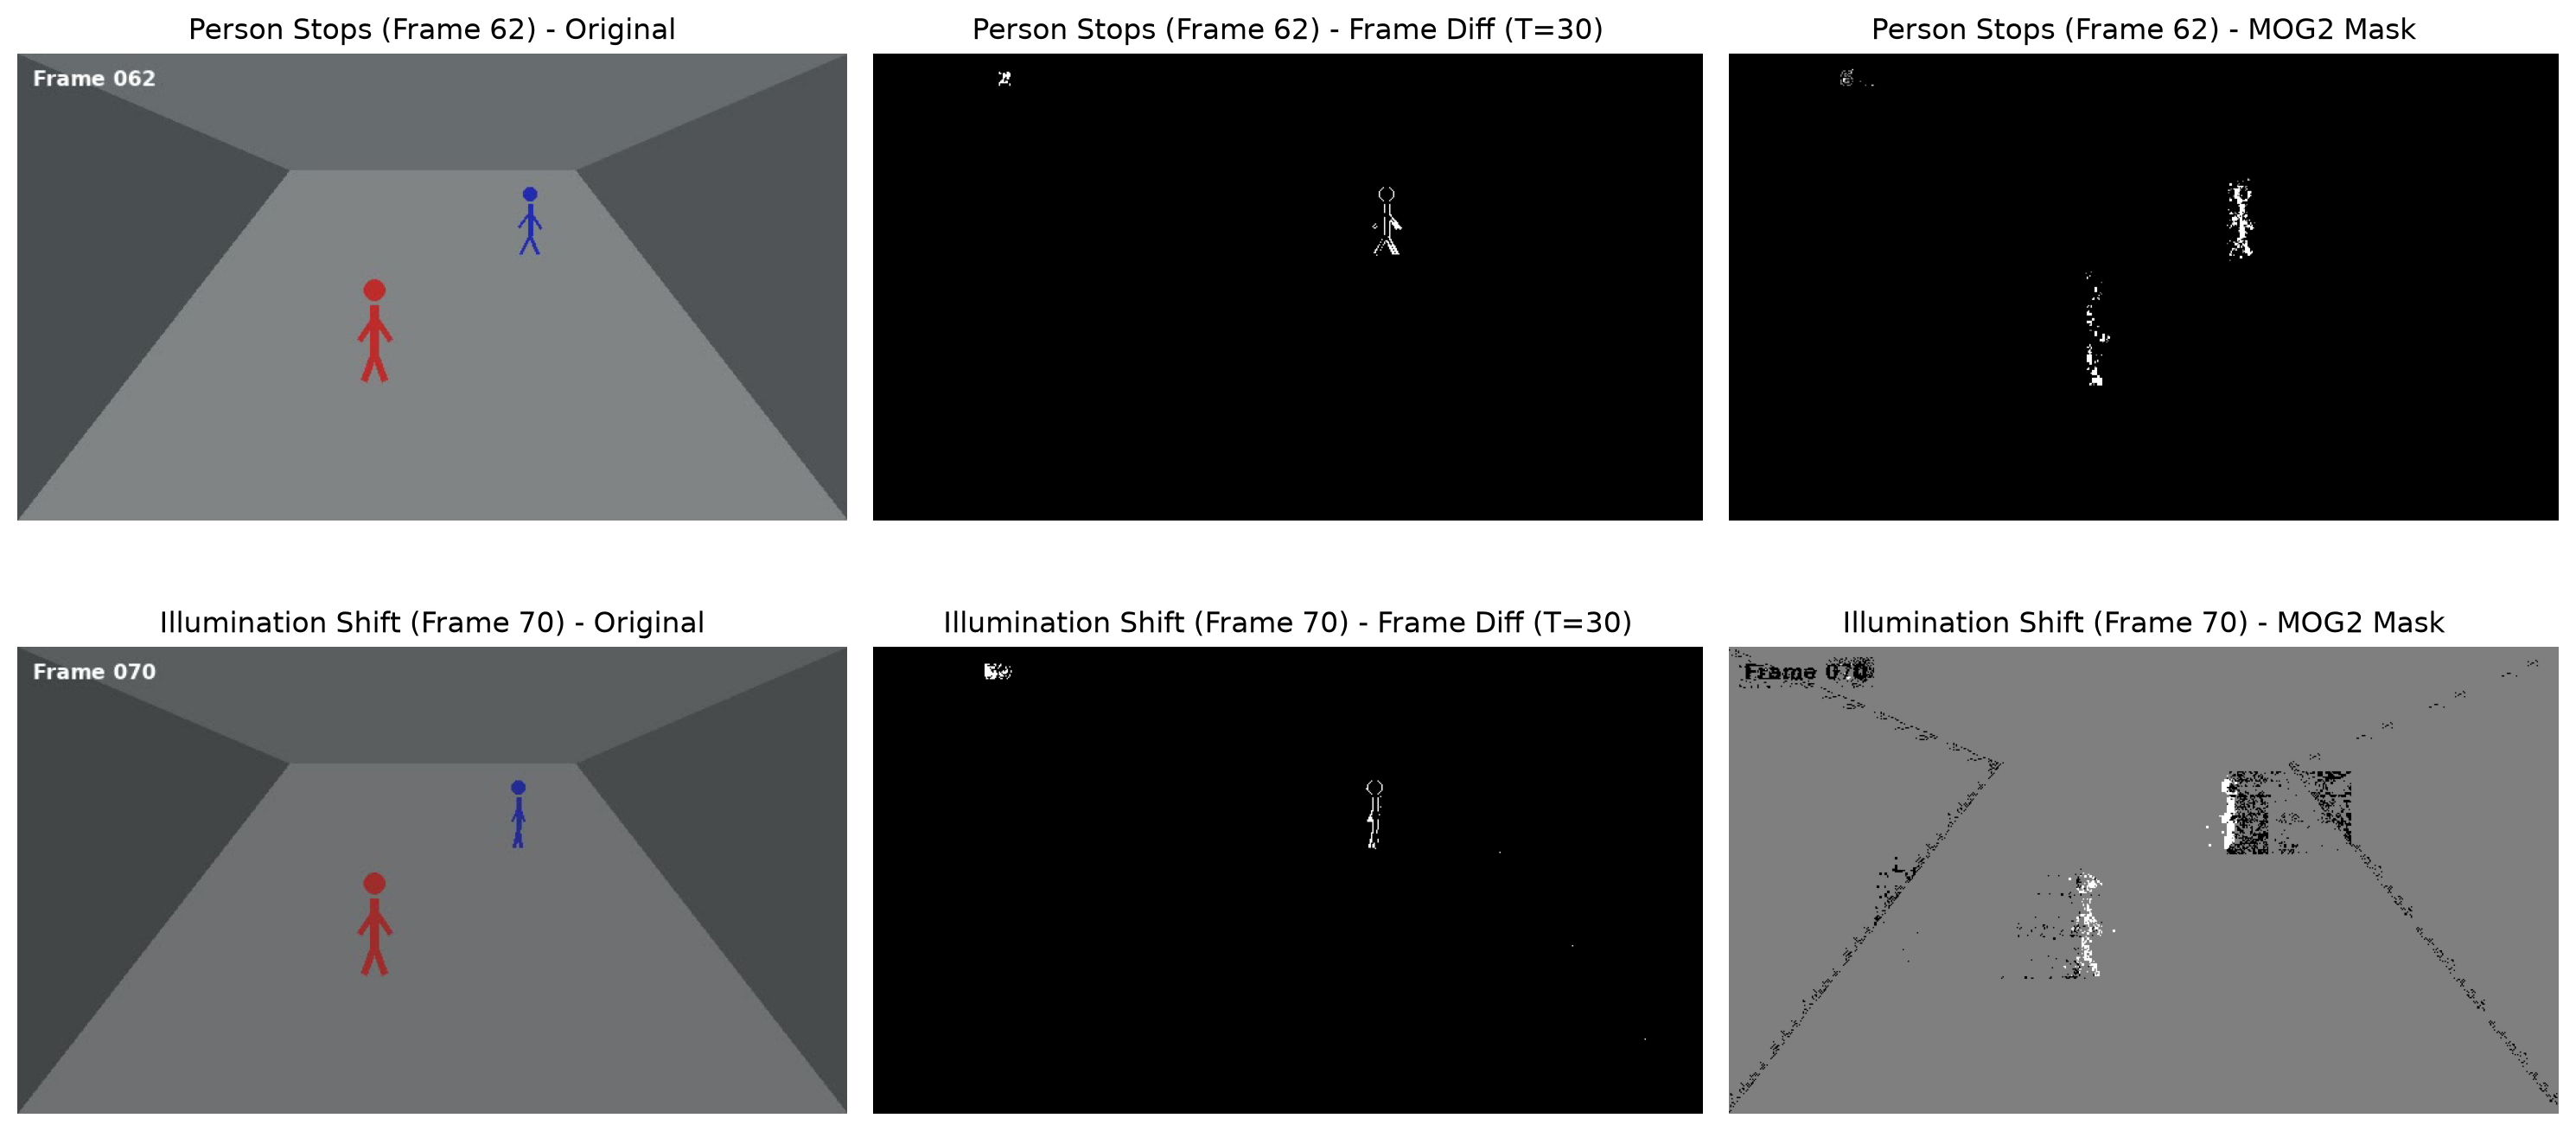
\includegraphics[width=0.98\textwidth]{images/failure_cases_comparison.png}
    \caption{Comparative analysis during critical failure segments: Stationary person (Frame 62) and Illumination change (Frame 70).}
    \label{fig:failure_comparison}
\end{figure}

\begin{table}[H]
\centering
\caption{Performance Comparison between Frame Differencing and MOG2}
\label{tab:comparison}
\begin{tabular}{p{3.2cm}p{6cm}p{6cm}}
\toprule
\textbf{Scenario} & \textbf{Frame Differencing} & \textbf{MOG2 Background Subtraction} \\
\midrule
Continuous Motion & Detects active contours and edges; hollow silhouettes. & Produces solid, dense foreground masks with shadow categorization. \\
\addlinespace
Stationary Subject (Frame 62) & \textbf{Fails immediately}: difference drops to zero, person vanishes from mask. & \textbf{Maintains detection briefly}, then gradually incorporates person into background model. \\
\addlinespace
Sudden Lighting Change (Frame 70) & Produces severe widespread false positives across the entire frame. & Triggers widespread false positives until Gaussian distributions readapt over history window. \\
\bottomrule
\end{tabular}
\end{table}

\subsection{Task 4: Motion Vector Estimation: Gradient, Magnitude, and Direction Representation}
To advance beyond binary motion masking, we compute continuous motion vector fields $(u, v)$ using Gunnar Farneback's dense optical flow algorithm and decompose vectors into polar magnitude $r$ and direction $\theta$.

\begin{figure}[H]
    \centering
    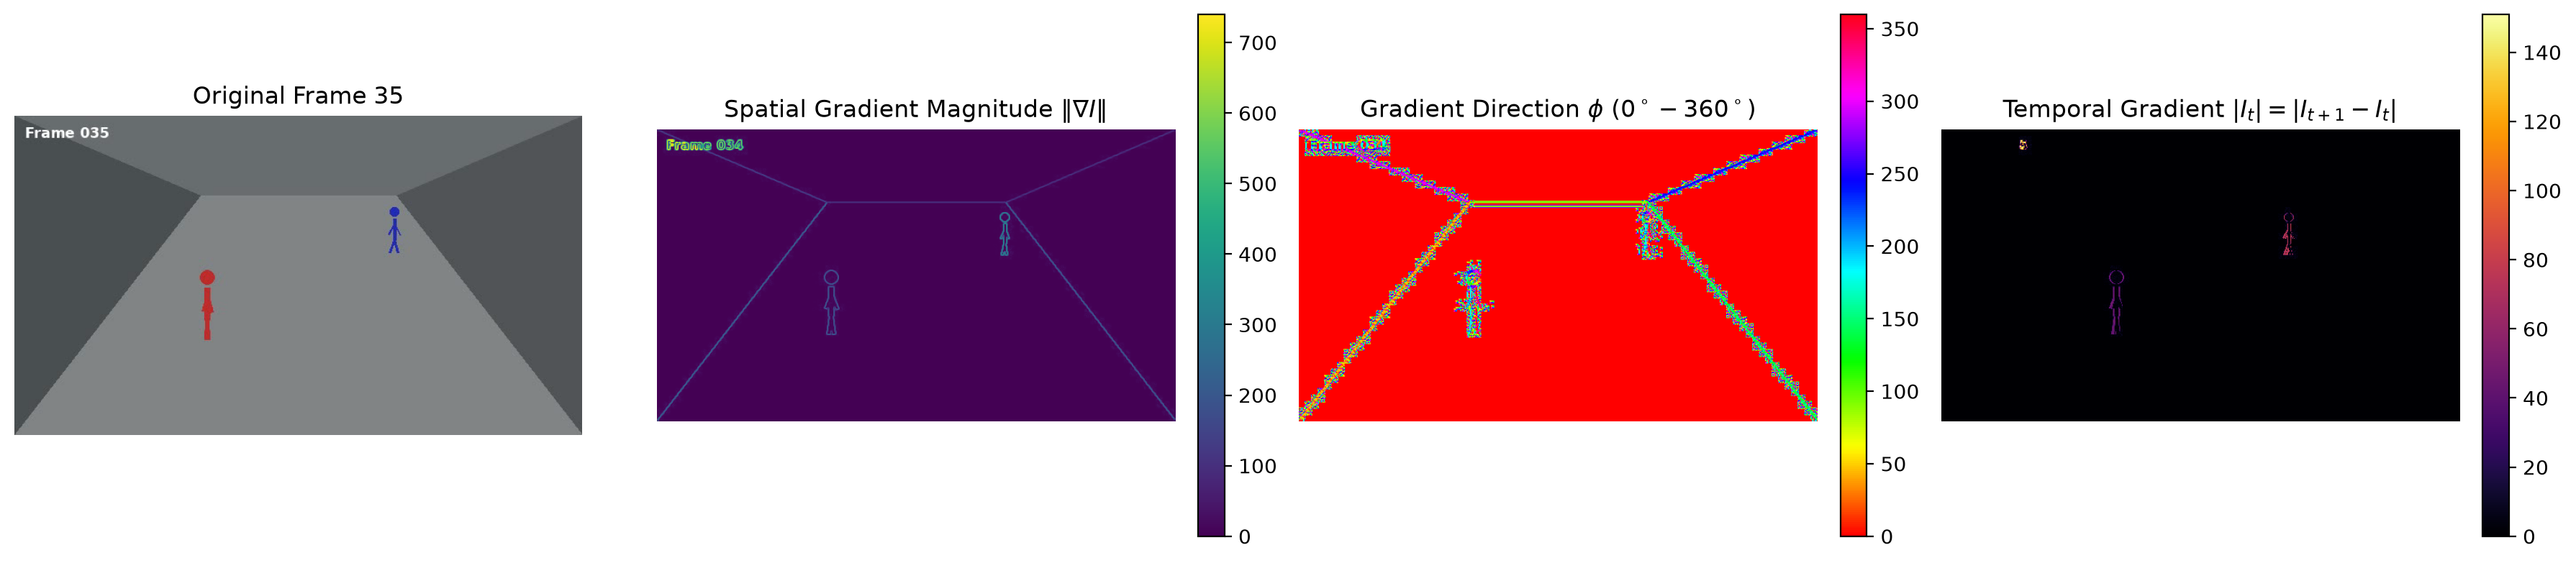
\includegraphics[width=0.98\textwidth]{images/motion_gradient_analysis.png}
    \caption{Spatial and temporal image gradient decomposition on Frame 35: Original Frame, Spatial Gradient Magnitude $\|\nabla I\|$, Gradient Direction $\phi$ ($0^\circ - 360^\circ$), and Temporal Gradient $|I_t|$.}
    \label{fig:motion_gradient}
\end{figure}

\begin{figure}[H]
    \centering
    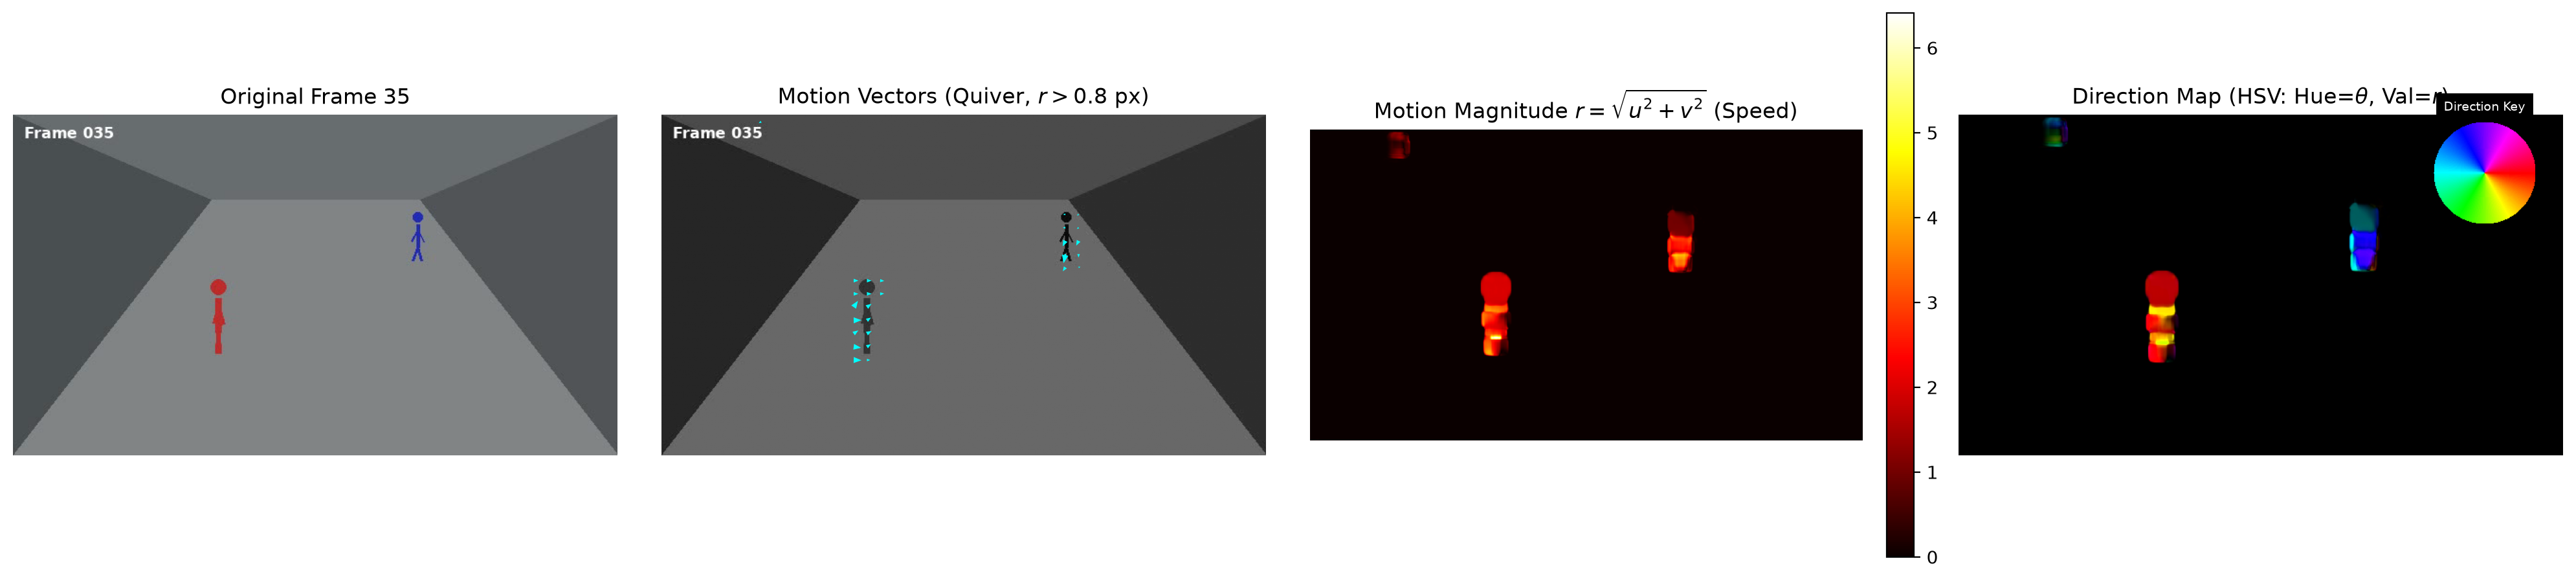
\includegraphics[width=0.98\textwidth]{images/optical_flow_quiver_hsv.png}
    \caption{Motion Vector Estimation and Directional Decomposition on Frame 35: Original Frame, Quiver Vector Field overlay ($r > 0.8$ px), Magnitude Heatmap (speed $r$), and Dense HSV Direction Map with circular direction key.}
    \label{fig:optical_flow_quiver_hsv}
\end{figure}

\begin{figure}[H]
    \centering
    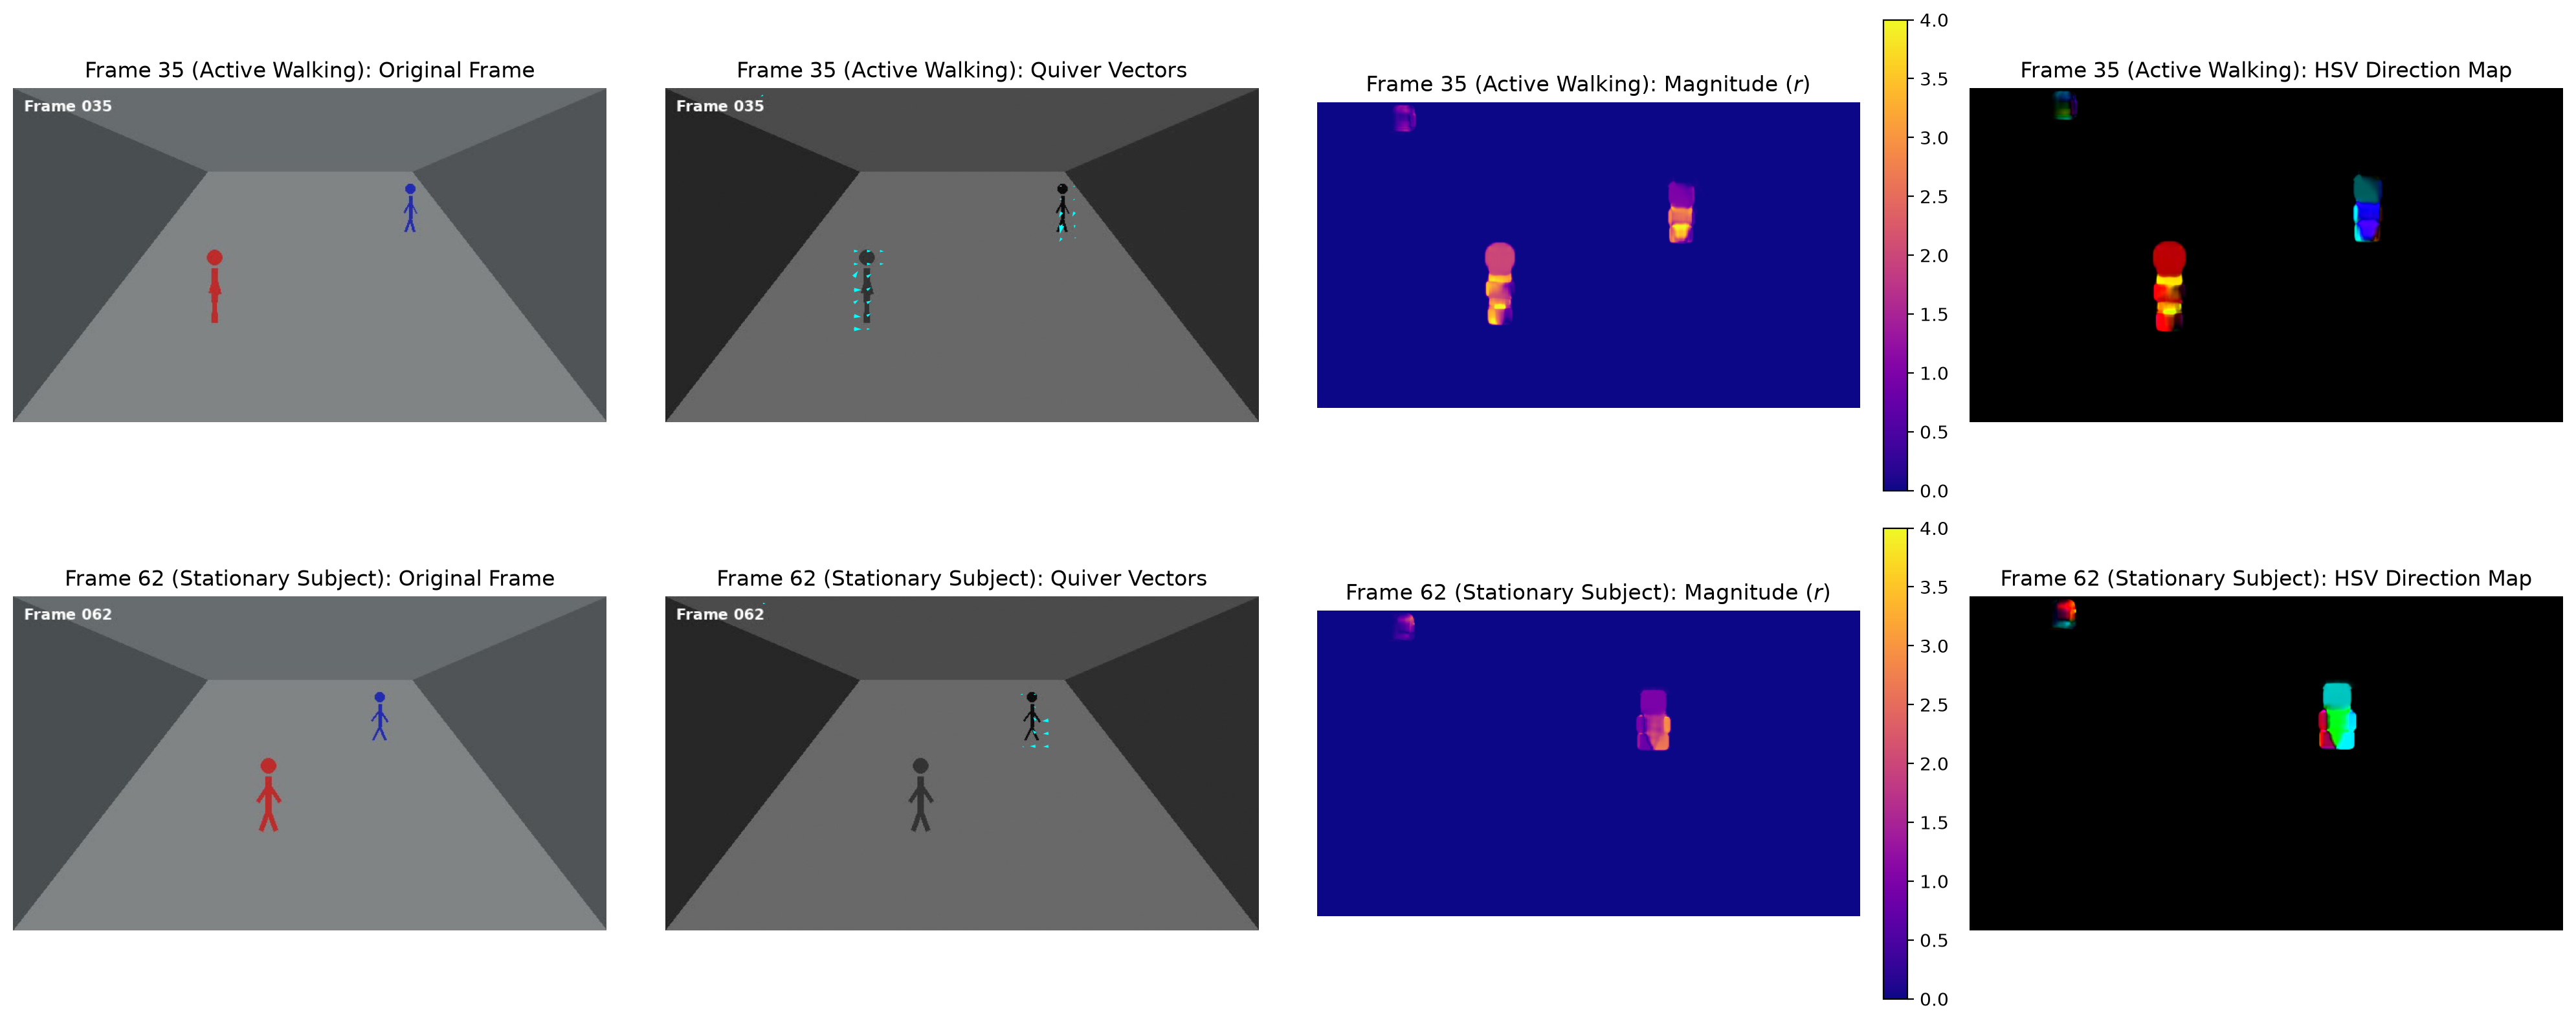
\includegraphics[width=0.98\textwidth]{images/motion_vector_moving_vs_paused.png}
    \caption{Evaluating Motion Vectors on Active Motion (Frame 35) vs. Paused Subject (Frame 62). While moving persons show prominent quiver vectors and saturated directional hues, the stationary person in Frame 62 exhibits zero velocity vectors ($r \approx 0$).}
    \label{fig:motion_vector_paused}
\end{figure}

\textbf{Key Observations from Motion Vector Representation:}
\begin{enumerate}
    \item \textbf{Directional Discernment:} In Frame 35, walking individuals moving across the hallway are clearly mapped to their respective direction headings. The dense HSV color wheel instantly identifies the trajectories of the subjects through distinct color hues (e.g., cyan/blue vs. green/yellow), which is completely lost in scalar frame differencing.
    \item \textbf{Speed Quantification:} Rather than binary thresholds, the magnitude map $r = \sqrt{u^2 + v^2}$ measures physical pixel displacement per frame, allowing exact velocity profiling.
    \item \textbf{Stationary Target Isolation:} In Frame 62, when the left person stops walking, optical flow vectors over their body drop below the threshold ($r < 0.8$ px), while the moving person on the right continues to exhibit active directional vectors.
\end{enumerate}

\section{Challenge Question and Discussion}

\subsection{Can a motion detector distinguish a stationary person from the background?}
\textbf{Answer:} \textbf{No.} Pure motion-based detectors (such as frame differencing and Gaussian mixture background subtractors) fundamentally rely on temporal pixel intensity variance over time. They lack semantic scene comprehension and cannot distinguish an unmoving human from a static background element once motion ceases.

\subsection{Limitations Evidenced in the Video}
\begin{enumerate}
    \item \textbf{Instant Blindness to Static Targets (Frame Differencing):} In Frame 62, the moment the left subject ceases moving, $|I_t - I_{t-1}| \approx 0$. The subject immediately disappears from the motion mask, yielding a false negative.
    \item \textbf{Background Absorption (MOG2):} Although MOG2 continues tracking the stationary person immediately after pausing, its adaptive learning rate causes the Gaussian mixture distribution to absorb stationary foreground pixels into the background model after a configurable number of frames.
    \item \textbf{Global Illumination Vulnerability:} In Frame 70, global light switching modifies pixel values globally, tricking both pixel-level difference and MOG2 models into marking entire walls and hallways as foreground.
\end{enumerate}

\subsection{Suggested Improvements}
\begin{enumerate}
    \item \textbf{Object Tracking and State Memory:} Couple the motion mask with a multi-object tracker (e.g., Kalman Filter or SORT). When a tracked bounding box velocity drops to zero, retain its state as \emph{"Stationary Person"} rather than discarding the track.
    \item \textbf{Semantic Deep Learning Detectors:} Integrate pre-trained object detectors (e.g., YOLOv8, SSD) that identify individuals using spatial visual feature representations rather than temporal changes.
    \item \textbf{Illumination-Invariant Representations:} Process frames in illumination-normalized color spaces (such as normalized chromaticity $r = R/(R+G+B), g = G/(R+G+B)$ or gradient/edge magnitude domains) to eliminate uniform ambient lighting shifts.
\end{enumerate}

\section{Conclusion}
In this lab assignment, we evaluated motion detection using Frame Differencing and MOG2 Background Subtraction on the corridor surveillance video. While both techniques effectively detect moving individuals under steady lighting, frame differencing fails immediately when a subject halts, and MOG2 eventually incorporates stationary subjects into its model. Sudden illumination shifts induce false positives in both approaches. Hybrid systems combining background modeling with object tracking and semantic object recognition are necessary for robust real-world surveillance.

\end{document}
